\documentclass{beamer}
\usepackage{amsmath, array, graphicx}
\usetheme{Warsaw}
\usecolortheme{default}

\title{LaTeX Course}
\author{Mikhail Borisov}
\institute{HSE}
\date{July 2022}

\begin{document}

\frame{\titlepage}

\AtBeginSection[]
{
  \begin{frame}
    \frametitle{Table of Contents}
    \tableofcontents[currentsection]
  \end{frame}
}

\begin{frame}
\frametitle{Table of Contents}
\tableofcontents
\end{frame}

\section{Random List}
\begin{frame}
\frametitle{Unordered Lists}
\begin{itemize}
    \item LaTex is pretty cool
    \item item 2
    \begin{itemize}
        \item wow, nested item
    \end{itemize}
\end{itemize}
\end{frame}

\section{Blocks}
\begin{frame}{Blocks}
In beamer you can make your text \alert{highlighted}. As well as create create blocks with texts

\begin{block}{Remark}
Sample text
\end{block}

\begin{alertblock}{Important theorem}
Sample text in red box
\end{alertblock}

\begin{examples}
Sample text in green box.
\end{examples}
\end{frame}


\section{Table}
\begin{frame}{Table}
    \resizebox{12cm}{!}{
    \begin{tabular}{|m{2cm}|m{2cm}|m{3cm}|m{4cm}|m{2cm}|m{4cm}|}
    \hline
     & Scaling & Unequal Scaling & Rotation & Horizontal Shear & Hyperbolic Rotation \\ \hline
     Illustration & 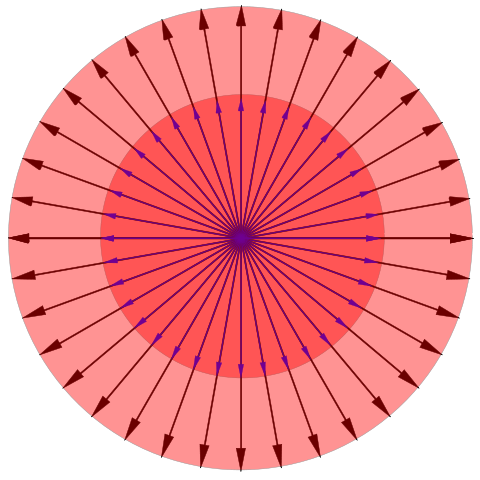
\includegraphics[width = 0.15\textwidth]{Images/480px-Homothety_in_two_dim.svg.png} & 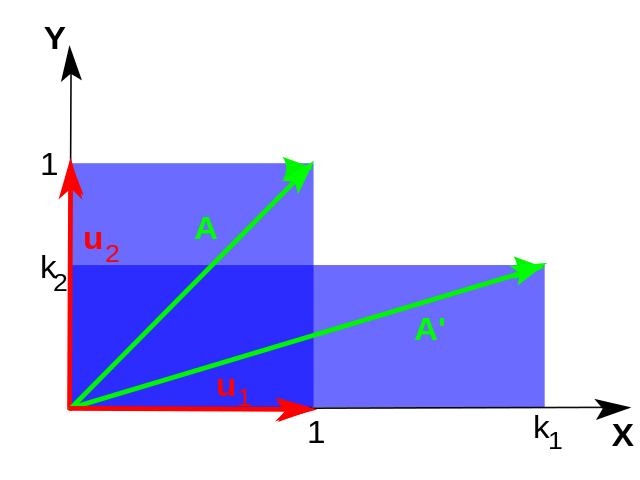
\includegraphics[width = 0.2\textwidth]{Images/640px-Unequal_scaling.svg.png} & 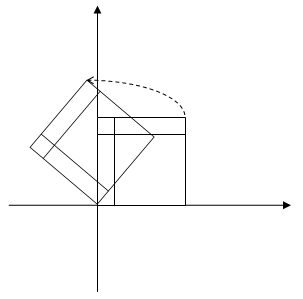
\includegraphics[width = 0.15\textwidth]{Images/Rotation.png} & 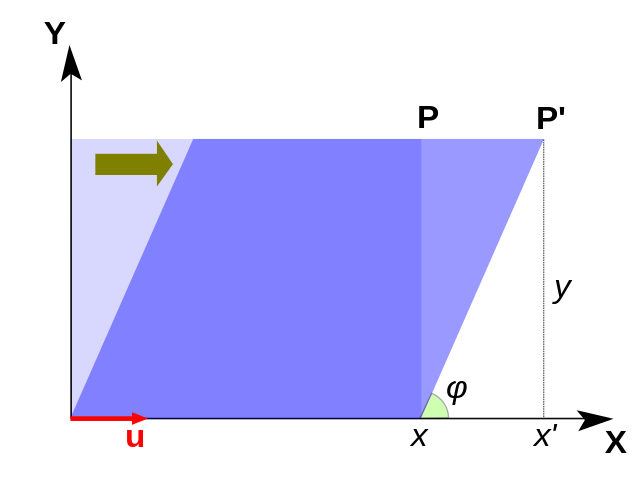
\includegraphics[width = 0.15\textwidth]{Images/640px-Shear.svg.png} & 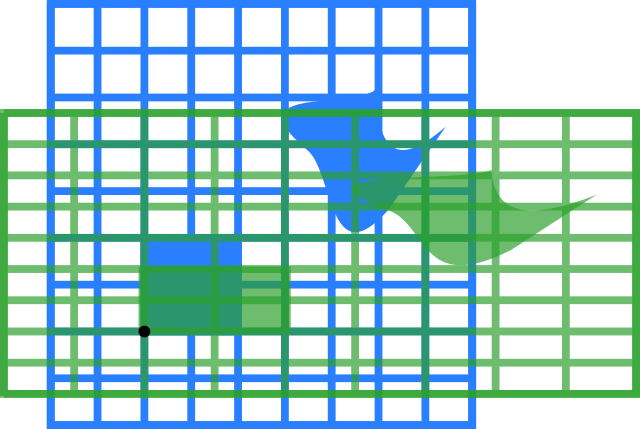
\includegraphics[width = 0.15\textwidth]{Images/640px-Squeeze_r=1.5.svg.png} \\ \hline
     Matrix & $\begin{bmatrix}
         k & 0 \\
         0 & k
         \end{bmatrix}$ & $\begin{bmatrix}
         k_1 & 0 \\
         0 & k_2
         \end{bmatrix}$ & $ \begin{bmatrix}
         \cos{\theta} & -\sin{\theta} \\
         \sin{\theta} & \cos{\theta}
         \end{bmatrix}$ & $\begin{bmatrix}
         1 & k \\
         0 & 1
         \end{bmatrix}$ & $\begin{bmatrix}
         \cosh{\varphi} & \sin{\varphi} \\
         \sin{\varphi} & \cosh{\varphi}
         \end{bmatrix}$\\ \hline
     Characteristic Polynomail & $(\lambda - k)^2$ & $(\lambda - k_1)(\lambda - k_2)$ & $\lambda^2 - 2\cos{\theta}\lambda + 1$& $(\lambda - 1)^2$ & $\lambda^2 - 2\cosh{\varphi}\lambda + 1$ \\ \hline
     Eigenvalues, $\lambda_i$ & $\lambda_1 = \lambda_2 = k$ & $\lambda_1 = k_1$ \newline $\lambda_2 = k_2$ & $\lambda_1 = e^{i\theta} = \cos{\theta} + i\sin{\theta}$ \newline $\lambda_2 = e^{-i\theta} = \cos{\theta} - i\sin{\theta}$ & $\lambda_1 = \lambda_2 = 1$ & $\lambda_1 = e^\varphi = \cosh{\varphi} + \sinh{\varphi}$ \newline $\lambda_2 = e^\varphi = \cosh{\varphi} - \sinh{\varphi}$ \\ \hline
     Algebraic multiplicity, $\mu_i = \mu(\lambda_i)$ & $\mu_1 = 2$ & $\mu_1 = 1$ \newline $\mu_2 = 1$ & $\mu_1 = 1$ \newline $\mu_2 = 1$ & $\mu_1 = 1$ & $\mu_1 = 1$ \newline $\mu_2 = 1$  \\ \hline
     Geometric multiplicity, $\gamma_i = \gamma(\lambda_i)$ & $\gamma_1 = 2$ & $\gamma_1 = 1$ \newline $\gamma_2 = 1$ & $\gamma_1 = 1$ \newline $\gamma_2 = 1$ & $\gamma_1 = 1$ & $\gamma_1 = 1$ \newline $\gamma_2 = 1$ \\ \hline
     Eigenvectors & All nonzero vectors & $\textbf{u}_1 = \begin{bmatrix}
         1 \\
         0
     \end{bmatrix}$ \newline $\textbf{u}_2 = \begin{bmatrix}
         0 \\
         1
     \end{bmatrix}$ & $\textbf{u}_1 = \begin{bmatrix}
         1 \\
         -i
     \end{bmatrix}$ \newline $\textbf{u}_2 = \begin{bmatrix}
         1 \\
         +i
     \end{bmatrix}$ & $\textbf{u}_1 = \begin{bmatrix}
         1 \\
         0
     \end{bmatrix}$  & $\textbf{u}_1 = \begin{bmatrix}
         1 \\
         1
     \end{bmatrix}$ \newline $\textbf{u}_2 = \begin{bmatrix}
         1 \\
         -1
     \end{bmatrix}$ \\ \hline
\end{tabular}
}
\end{frame}

\begin{frame}{The End}
\centering
The End
    
\end{frame}

\end{document}